\documentclass[a4paper]{article}

%% Language and font encodings
\usepackage[english]{babel}
\usepackage[utf8]{inputenc}
\usepackage[T1]{fontenc}

%% Sets page size and margins
\usepackage[a4paper,top=3cm,bottom=2cm,left=3cm,right=3cm,marginparwidth=1.75cm]{geometry}

%% Useful packages
\usepackage{amsmath}
\usepackage{graphicx}
\usepackage[colorinlistoftodos]{todonotes}
\usepackage[colorlinks=true, allcolors=blue]{hyperref}
\usepackage{floatrow}
\usepackage{float}
\usepackage{subcaption}
\usepackage{booktabs}
\usepackage{color}
\usepackage{tikz}
\usepackage{titlesec}
\usepackage{caption}
\usetikzlibrary{shapes.geometric, arrows}

% package to manage citations
\usepackage[backend=bibtex,style=authoryear-comp,sorting=nyt,isbn=false,url=false, natbib=true]{biblatex}
\addbibresource{references.bib}

\tikzstyle{startstop} = [rectangle, rounded corners, minimum width=3cm, minimum height=1cm,text centered, draw=black,text width = 5cm, fill=red!30]
\tikzstyle{io} = [trapezium, trapezium left angle=70, trapezium right angle=110, minimum width=3cm, minimum height=1cm, text centered, draw=black, fill=blue!30]
\tikzstyle{process} = [rectangle, minimum width=3cm, minimum height=1cm, text centered, text width = 4cm, draw=black, fill=orange!30]
\tikzstyle{decision} = [diamond, minimum width=2cm, minimum height=1cm,text centered,text width = 2.5cm, draw=black, fill=green!30]
\tikzstyle{arrow} = [thick,->,>=stealth]

\definecolor{ErasmusBlue}{RGB}{12, 32, 116}

%Use 4 levels of sections using package titlesec
\setcounter{secnumdepth}{4}
\newcommand{\subsubsubsection}[1]{\paragraph{#1}\mbox{}\\\\}

\newcommand{\argmax}[1]{\underset{#1}{\operatorname{arg}\,\operatorname{max}}\;}

\begin{document}
\title{PRIAS Personalized Biopsy Schedules}

\author{Firstname1 Lastname1}

\date{}

\maketitle

% !TEX root =  ../main_manuscript.tex 
\begin{abstract}
\texttt{Objective}: To develop a model and methodology for predicting the risk of Gleason \emph{upgrading} in prostate cancer active surveillance (AS) patients, and using the predicted risks to create risk-based \emph{personalized} biopsy schedules as an alternative to one-size-fits-all schedules (e.g., annually). Furthermore, to assist patients and doctors in making shared decisions of biopsy schedules, by providing them quantitative estimates of the \emph{burden} and \emph{benefit} of opting for personalized versus any other schedule in AS. Last, to externally validate our model and implement it along with personalized schedules in a ready to use web-application.\\

\texttt{Materials and Methods}: We used longitudinal prostate-specific antigen (PSA) measurements, timing and results of previous biopsies, and age at baseline from the world's largest AS study, Prostate Cancer Research International Active Surveillance or PRIAS (7813 patients, 1134 experienced upgrading). We fitted a Bayesian joint model for time-to-event and longitudinal data to the PRIAS dataset. We then externally validated our model in the largest six AS cohorts of the Movember Foundation's Global Action Plan (GAP3) database (${>20,000}$ patients, 27 centers worldwide), covering nearly 73\% of all GAP3 patients. We used the predicted upgrading-risks from the validated models to schedule biopsies whenever a patient's risk of upgrading was above a certain threshold. To assist patients in choice of this threshold to compare the resulting schedule with currently practiced schedules, we provided them the timing and the total number of biopsies (burden) planned, and the predicted time delay in detecting upgrading (shorter is better) for each schedule.\\

\texttt{Results}: The cause-specific cumulative upgrading-risk at year five of follow-up was 35\% in PRIAS, and at most 50\% in GAP3 cohorts. In the PRIAS based model, PSA velocity was a stronger predictor of upgrading (Hazard~Ratio:~2.47, 95\%CI:~1.93--2.99) than PSA value (Hazard~Ratio:~0.99, 95\%CI:~0.89--1.11). Our model had a moderate area under the receiver operating characteristic curve (0.6--0.7) in validation cohorts. The prediction error was moderate (0.1--0.2) in GAP3 cohorts where the impact of PSA value and velocity on upgrading-risk was similar to PRIAS, but large (0.2--0.3) otherwise. Our model required recalibration of baseline upgrading-risk in validation cohorts. We used predicted upgrading-risk from the validated model to create personalized biopsy schedules for real AS patients and implemented them in a web-application (\url{http://tiny.cc/biopsy}).\\

\texttt{Conclusions}: We successfully developed and validated a model for predicting upgrading-risk, and providing risk-based personalized biopsy decisions, in prostate cancer AS. Personalized prostate biopsies are a novel alternative to fixed one-size-fits-all schedules that may help to reduce unnecessary prostate biopsies while maintaining cancer control. The model and schedules made available via a web-application enable shared decision making of biopsy schedules by comparing fixed and personalized schedules on total biopsies and expected time delay in detecting upgrading.
\end{abstract}
% !TEX root =  ../main_manuscript.tex 
\section{Introduction}
\label{sec:introduction}
Chronic non-communicable diseases (e.g., cancer, renal, cardiovascular diseases, etc.) are the primary cause of human deaths worldwide~\citep{alwan2010monitoring}. After diagnosis, in many such patients, surveillance tests are performed periodically to detect disease \textit{progression}, a non-terminal event. Often the most accurate or gold standard surveillance tests are also invasive. For example, to diagnose progression, biopsies are conducted repeatedly in prostate cancer~\citep{bokhorst2015compliance}, endoscopies in Barrett's esophagus~\citep{streitz1993endoscopic}, and colonoscopies in colorectal cancer~\citep{krist2007timing}. Repeat biopsies are also utilized to detect allograft deterioration in lung~\citep{mcwilliams2008surveillance} and kidney transplant~\citep{henderson2011surveillance} patients.

Usually, invasive tests are scheduled in a fixed manner, e.g., every six months. Test frequency varies between diseases~\citep{henderson2011surveillance,bokhorst2015compliance,krist2007timing} and cohorts. Although, due to the periodical nature of test schedules, progression is always detected with a time delay (Figure~\ref{fig:delay_explanation}). This time delay can be reduced by scheduling tests frequently. However, invasive tests are difficult to conduct, can lead to severe complications~\citep{loeb2013systematic,krist2007timing}, cause patient discomfort, and sometimes patients may not comply with frequent tests~\citep{bokhorst2015compliance}. In this regard, fixed test schedules ignore the differences in speed of progression between patients, and impose an equal medical burden on all. Hence, the frequency of invasive tests holds important implications for patients.

\begin{figure}
\centerline{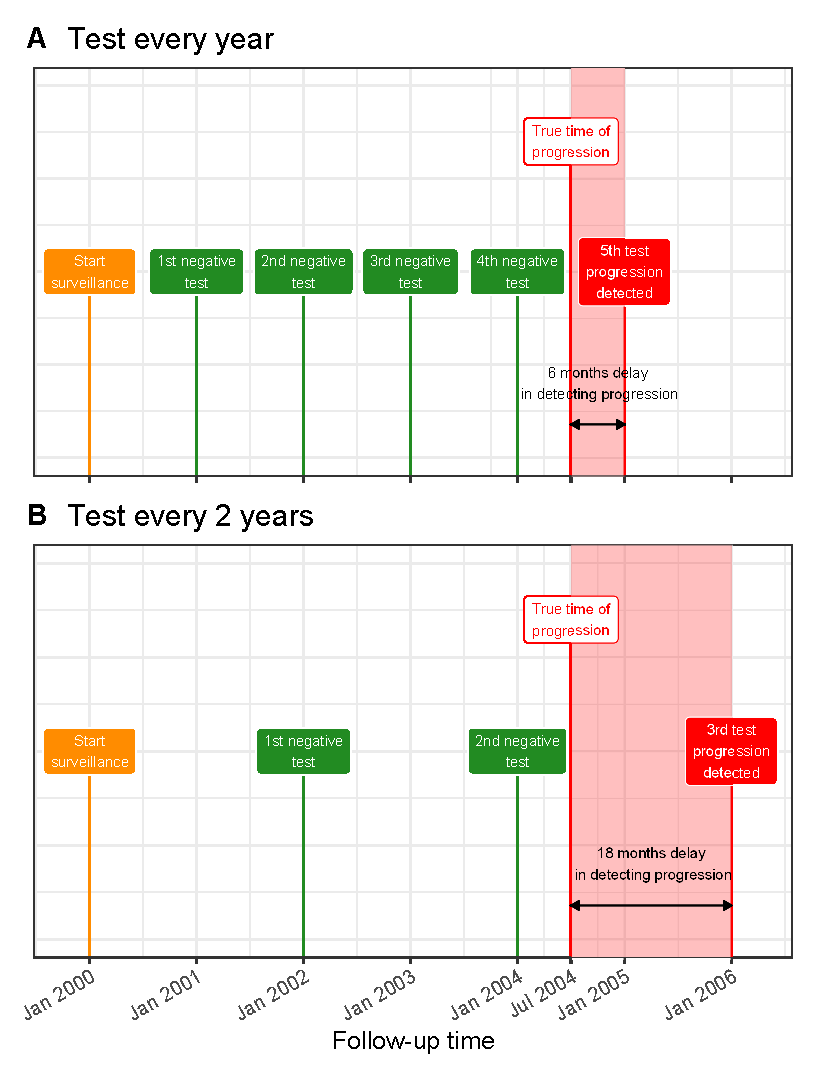
\includegraphics{images/delay_explanation.eps}}
\caption{\textbf{Trade-off between the number of invasive tests and time delay in detecting progression (non-terminal event of interest):} The true time of progression for this patient July 2004. More frequent invasive tests in \textbf{Panel~A} lead to a smaller time delay in detection of progression than less frequent invasive tests in \textbf{Panel~B}. Since invasive tests are conducted periodically, the time of progression is observed as an interval. For example, between Jan~2004--Jan~2005 in \textbf{Panel~A} and between Jan~2004--Jan~2006 in \textbf{Panel~B}.} 
\label{fig:delay_explanation}
\end{figure}

In this paper, we aim to balance the number of invasive tests (burden) and the time delay in detection of \textit{progression} (less is beneficial) better than fixed schedules. For this purpose, we intend to create personalized test schedules that exploit patient-specific clinical data accumulated during follow-up. This data includes baseline characteristics of patients; results from previous invasive tests; and longitudinal biomarker, physical examination, and medical imaging measurements, etc. Previous approaches for personalized schedules may be divided into three categories. First, heuristic methods such as decision making flowcharts, e.g.,~\citet{bokhorst2015compliance}. However, flowcharts discretize continuous clinical outcomes, often utilize only the latest data point, and ignore the measurement error in observed outcomes. Second, personalized test decisions employing partially observable Markov decision processes~\citep{alagoz2010operations, steimle2017markov}. Although, their application with continuous outcomes is limited by the curse of dimensionality. Third, personalized schedules obtained by optimizing a loss function of clinical parameters of interest~\citep{bebu2017optimal,rizopoulos2015personalized}, including our previous work on scheduling biopsies in prostate cancer~\citep{tomer2019personalized}. In this work, we will employ the third approach.

First, we develop a full specification of the joint distribution of patient-specific longitudinal clinical outcomes and time of \textit{progression}. We achieve this using joint models for time-to-event and longitudinal data~\citep{tsiatis2004joint,rizopoulos2012joint}. We use joint models because they are inherently personalized. Specifically, they exploit patient-specific random effects~\citep{laird1982random} to model longitudinal outcomes without discretizing them. We subsequently employ the fitted joint model for new patients, to estimate their patient-specific cumulative-risk over their current and future follow-up visits. These risk predictions utilize their clinical data accumulated until their latest follow-up. We then schedule invasive tests on all those future follow-up visits where a patient's conditional cumulative-risk of progression is above a certain threshold (e.g., 10\% risk). We also automate the choice of this threshold and the resulting schedule. More specifically, we optimize a function of the number of tests in a schedule and the expected time delay in the detection of progression. We estimate this delay in a patient-specific manner for both fixed and personalized schedules, thus facilitating shared-decision making of invasive test schedules.

This research is motivated by the problem of scheduling biopsies~\citep{nieboer2018active} in the world's largest prostate cancer active surveillance study PRIAS~\citep{bokhorst2015compliance}. It has 7813 patients, 104904 longitudinal measurements, and 1134 patients with cancer progression. Patients in PRIAS have low and very-low grade prostate cancer, often over-diagnosed due to prostate-specific antigen (PSA) based screening tests~\citep{crawford2003epidemiology}. The goal of surveillance is to delay serious treatments (e.g., surgery, chemotherapy, etc.) until cancer progression is observed. For this purpose, patients are monitored continually via PSA (ng/mL) blood tests, digital rectal examination (DRE) for shape and size of the tumor, and biopsy Gleason grade group~\citep{epsteinGG2014}. The latter is the strongest indicator of cancer-related outcomes. Consequently, treatment is commonly advised upon observing an increase in a patient's biopsy Gleason grade group (cancer progression). Currently, the most common biopsy schedule of yearly biopsies~\citep{loeb2014heterogeneity} leads to many unnecessary biopsies in slow/non-progressing patients (50\% proportion in some cohorts). Biopsy burden combined with patient non-compliance to frequent biopsies~\citep{bokhorst2015compliance} has raised concerns regarding the optimal biopsy schedule. Since prostate cancer has the second highest incidence among all cancers in males~\citep{GlobalCancerStats2012}, biopsy schedules tailored for individual patients can reduce the overall burden of biopsies in a large number of patients worldwide.

The rest of the paper is as follows. Section~\ref{sec:jointmodel} briefly introduces the joint modeling framework. In Section~\ref{sec:schedule} we present the methodology for personalized schedules, and then demonstrate them for biopsies in real PRIAS patients in Section~\ref{sec:results}. Lastly, in Section~\ref{sec:sim_study} we show the efficacy of personalized schedules via a realistic simulation study based on PRIAS patients.
% !TEX root =  ../main.tex 

\section{A framework for personalized biopsy schedules}
\label{sec : framework_pers_biop_sched}
The first step in creating a personalized schedule for biopsies is to come up with a model for Gleason scores, PSA levels and other subject specific characteristics. In PRIAS, PSA levels are measured at the time of induction, every 3 months for the first 2 years in the study and then every 6 months thereafter. Thus PSA levels can be modeled as a longitudinal outcome. As mentioned earlier, patients in PRIAS have a Gleason score of 6 or less at the time of induction in the study, and patients are removed from AS the first time Gleason reclassification takes place. Since our interest also lies in time to Gleason reclassification, we model it as a time to event outcome. i.e. time to Gleason reclassification. While univariate modeling of the two aforementioned outcomes can be done separately using longitudinal model and survival models, it is important to note that they are not independent. To model the association between the two types of outcomes we use a joint model for time to event and longitudinal outcomes.

\subsection{Joint model for Gleason reclassification and PSA levels}
\label{subsec : jm_definition}
Let $T_i^*$ denote the true Gleason reclassification time for the $i^{th}$ subject. Let the times at which biopsies are conducted for the $i^{th}$ patient be denoted by $C_i = \{C_{i0}, C_{i1}, ... C_{ig_i}; C_{ij} < C_{ik}, \forall j<k \}$. $T_i^*$ cannot be observed directly and it is only known that it falls in an interval $(l_i, r_i]$, where $l_i = C_{i(g_i-1)}, r_i = C_{ig_i}$ if Gleason reclassification is observed and $l_i = C_{ig_i}, r_i=\infty$ if patient drops out. The latter is also known as right censoring. Let $\boldsymbol{y}_i$ denote the $n_i \times 1$ longitudinal outcome vector for the PSA levels of the $i^{th}$ subject. The population of interest is all the patients enrolled in AS. For a sample of $n$ patients from this population the complete data is denoted by $\mathcal{D}_n = \{T_i, l_i, r_i, \boldsymbol{y}_i; i = 1,...n\}$, where $T_i \epsilon (l_i, r_i]$ denotes the observed time of Gleason reclassification.\\

To model the evolution of the longitudinal outcome, which is PSA levels in the case at hand, the joint model utilizes a linear mixed effects model. The longitudinal outcome $y_i(t)$ at time $t$ is modeled as:

\begin{equation*}
\begin{split}
y_i(t) &= m_i(t) + \varepsilon_i(t), \\
&= \boldsymbol{x}_i^T(t) \beta + \boldsymbol{z}_i^T(t) \boldsymbol{b}_i + \varepsilon_i(t)
\end{split}
\end{equation*}
%Do not introduce a space here, otherwise it starts a new paragraph
where, $m_i(t)$ denotes the true and unobserved value of the longitudinal outcome at time $t$. $\varepsilon_i(t) \sim N(0, \sigma^2)$ denotes the measurement error term, assumed normally distributed with variance $\sigma^2$. $\beta$ denotes the vector of the unknown fixed-effects parameters. $\boldsymbol{b}_i \sim N(0, \boldsymbol{D})$ denotes the vector of random effects, assumed normally distributed with mean zero and covariance matrix D, and independent of $\varepsilon_i(t)$. $\boldsymbol{x}_i(t)$ and $\boldsymbol{z}_i(t)$ denote row vectors of the design matrices for the fixed and random effects, respectively. For non continuous longitudinal outcomes joint models utilize Generalized linear mixed models \citep{rizopoulos2012joint}.\\

Since both PSA levels and Gleason scores are affected by the state of prostate cancer, they are inherently correlated with each other. To this end, the joint model utilizes a relative risk sub-model where the hazard of Gleason reclassification $h_i(t)$ at any time point $t$ depends on the history of true and unobserved values of PSA levels $\mathcal{M}_i(t) = \{m_i(v), 0\leq v \leq t\}$ measured up to that time point. Joint models offer flexibility in modeling this dependence. In its simplest form, the hazard may depend on instantaneous value of PSA $m_i(t)$ at time $t$. More sophisticated ones are dependence of hazard at time $t$ on PSA-DT, PSA velocity $m'_i(t) = \dfrac{d m_i(t)}{dt}$, or even on the cumulative effect of PSA $\int_0^t m_i(s) \,ds$ up to $t$. The fact that any functional form of dependence is possible, is evident from the following equation:

\begin{equation*}
h_i(t \mid M_i(t), \boldsymbol{w}_i) = h_0(t) e^{\gamma^T\boldsymbol{w}_i + f\{M_i(t), \boldsymbol{b}_i, \alpha\}}
\end{equation*}
where $h_0(t)$ is the baseline hazard at time $t$. $\boldsymbol{w}_i$ is a vector of baseline covariates and $\gamma$ are the corresponding parameters. The function $f(\cdot)$ parametrized by vector $\alpha$ specifies the features of longitudinal outcome that are are included in the linear predictor of the relative risk model.\\

While $\alpha$ controls the strength of association between the hazard of reclassification and features of the PSA levels, the fact that both Gleason scores and PSA levels are internally related to a patient's health, is manifested by the random effects $\boldsymbol{b}_i$ in the model. The joint model postulates that given the random effects, time to Gleason reclassification and PSA levels measured at different time points are mutually independent. As mentioned earlier, in PRIAS study PSA-DT is used to decide the schedule of biopsies. Although PSA-DT is computed using observed PSA values, dependence on observed longitudinal history $\mathcal{Y}(t) = \{y_i(v), 0\leq v \leq t\}$ at any time $t$, is not the same as dependence on patient's health. This because dependence on patient's health, manifested by $\boldsymbol{b}_i$ is same as dependence on future unobserved values of PSA. Thus the inference for the parameters of interest $\theta$ doesn't change even if uncertainty in biopsy schedule $C_i$ is not modeled. The kernel of the corresponding joint likelihood conditional on the random effects and the model parameters is given by:

\begin{equation*}
p(T_i, l_i, r_i, \boldsymbol{y}_i \mid \boldsymbol{b}_i, \theta) \propto p(T_i \mid l_i, r_i, \boldsymbol{b}_i, \theta) p(\boldsymbol{y}_i \mid \boldsymbol{b}_i, \theta)
\end{equation*}

\subsection{Personalized scheduling approaches}
\label{subsec : pers_sched_approaches}
Once a joint model for Gleason reclassification and PSA levels is obtained, the next step is to use it to create personalized schedules for biopsies. In this section we present the various personalized biopsy scheduling approaches and their motivation. The personalized schedules that we propose are dynamic in nature and thus at any given time, only 1 future biopsy is scheduled. The age of the patient and entire PSA, repeat biopsy history up to that time point is considered while computing the time of next biopsy. To elucidate the scheduling methods, let us assume that the a personalized schedule is to be created a new patient numbered $j$ who is not present in the original sample of patients $\mathcal{D}_n$. Further let us assume that the patient did not have a Gleason reclassification at their last biopsy, performed at time $t$ and that the PSA measurements are available for the patient up to a time point $s > t$. Combining these two pieces of information, the predictive distribution $g(T^*_j)$ for time to Gleason reclassification for this patient is given by (conditioning on baseline covariates $\boldsymbol{w}_i$ is dropped for notational simplicity here onwards):

\begin{equation}
\label{eq : dyn_dist_fail_time}
\begin{split}
g(T^*_j) &= p(T^*_j \mid T^*_j > t, \mathcal{Y}_j(s), \mathcal{D}_n)\\
%&= \int p(T^*_j \mid T^*_j > t, \mathcal{Y}_j(s), \theta) p(\theta \mid \mathcal{D}_n) \,d\theta\\
%&= \int \int p(T^*_j \mid T^*_j > t, \mathcal{Y}_j(s), \boldsymbol{b_j}, \theta) p(\boldsymbol{b}_j \mid T^*_j>t, \mathcal{Y}_j(s), \theta)p(\theta \mid \mathcal{D}_n) \,d\boldsymbol{b}_j \,d\theta
\end{split}
\end{equation}
where $\mathcal{Y}_j(s)$ denotes the history of PSA measurements done up to time $s$. Given the predictive distribution, our goal is find the optimal time $u \geq s$ of the next biopsy. To achieve this we use principles from statistical decision theory in a Bayesian setting \citep{bergerDecisionTheory,robertBayesianChoice}. More specifically, we propose to choose future biopsy time $u$ by minimizing the posterior expected loss $E_g[L(T^*_j, u)]$, where the expectation is taken w.r.t. the predictive distribution $g(T^*_j)$. 

\begin{equation*}
E_g[L(T^*_j, u)] = \int_t^\infty L(T^*_j, u) p(T^*_j \mid T^*_j > t, \mathcal{Y}_j(s), \mathcal{D}_n) \,dT^*_j
\end{equation*}
Various loss functions $L(T^*_j, u)$ have been proposed in literature \citep{robertBayesianChoice}. We next present the loss functions we use in this work and the motivation for their choice.

\subsubsection{Expected time of Gleason reclassification}
\label{subsubsec : exp_fail_time}
One of the reasons, patients did not comply with the existing PRIAS schedule was \textquoteleft complications on a previous biopsy \textquoteright. Therefore, it makes sense to have as less biopsies as possible. In the ideal case only 1 biopsy, performed at the exact time of Gleason reclassification is sufficient. In this regard, the squared loss function $L(T^*_j, u) = (T^*_j - u)^2$ has the property that the loss increases quadratically as the error $T^*_j - u$ increases. So the squared loss function satisfies our requirement of choosing a $u$ as close to the true Gleason reclassification time as possible. The posterior expected loss is given by:

\begin{equation}
\label{eq : posterior_squared_loss}
\begin{split}
E_g[L(T^*_j, u)] &= E_g[(T^*_j - u)^2]\\
&=E_g[(T^*_j)^2] + u^2 -2uE_g[T^*_j]
\end{split}
\end{equation}
The posterior expected loss in equation \ref{eq : posterior_squared_loss} attains its minimum at $u = E_g[T^*_j]$, also known as expected time of Gleason reclassification.

\subsubsubsection{Estimation}
Since there is no closed form solution available for $E_g[T^*_j]$, for its estimation we introduce a construct called dynamic survival probability \citep{rizopoulos2011dynamic}. The dynamic survival probability $\pi_j(v \mid t, s)$ of patient $j$ is the survival probability at time $v$, conditional on the observed PSA history $\mathcal{Y}_j(s)$ and the fact that the patient did not have Gleason reclassification up to $t$. It is given by:

\begin{equation}
\pi_j(v \mid t, s) = Pr(T^*_j \geq v \mid  T^*_j >t, \mathcal{Y}_j(s), D_n), v \geq t
\end{equation}
The relationship between expected time of Gleason reclassification and dynamic survival probability is given by:

\begin{equation*}
E_g[T^*_j] = t + \int_t^\infty \pi_j(v \mid t, s) \,dv
\end{equation*}
Since the R package JMbayes already provides an implementation of $\pi_j(v \mid t, s)$, this approach was preferred over Monte Carlo methods to estimate $E_g[T^*_j]$ from the predictive distribution $g(T^*_j)$. A limitation of expected time of Gleason reclassification though, is that it is only useful when the variance of predictive distribution $g(T^*_j)$ is small. The variance is given by:

\begin{equation}
\begin{split}
Var_g[T^*_j] &= E_g[{T^*_j}^2] - {E_g[T^*_j]}^2\\
&= 2 \int_t^\infty {(v-t) \pi_j(v \mid t, s) \,dv} - {\bigg(\int_t^\infty \pi_j(v \mid t, s) \,dv\bigg)}^2
\end{split}
\end{equation}
It is to be noted that the posterior expected loss with the squared loss function is equal to the variance. Since the variance is same as expected loss....loss increases....intuitive??
\textcolor{red}{\textbf{THEORETICALLY PROVE HOW VARIANCE DECREASES WITH LESS Y(s)}}

\subsubsection{Dynamic risk of reclassification}
\label{subsubsec : dynamic_risk_definitions}
In a practical scenario it is possible that a doctor or a patient may not want to exceed a certain risk of reclassification $1 - \pi_j(u \mid t, s)$ since the last biopsy. The personalized scheduling approach based on dynamic risk of reclassification, schedules the next biopsy at a time point $u$ such that the dynamic risk of reclassification is higher than a certain threshold $1-\kappa,\ \kappa \epsilon [0,1]$ beyond $u$. Or in other words the dynamic survival probability $\pi_j(u \mid t, s)$ is below a threshold $\kappa$ beyond $u$. In this regard, the posterior expected loss for the following multilinear loss function can be minimized to find the most optimal $u$:

\begin{equation}
\label{eq : loss_dynamic_risk}
L_{k_1, k_2}(T^*_j, u) =
    \begin{cases}
      k_2(T^*_j-u) & if(T^*_j > u)\\
      k_1(u-T^*_j) & \text{otherwise}
    \end{cases}       
\end{equation}
where $k_1 > 0$, $k_2 > 0$ are constants parameterizing the loss function. The posterior expected loss function $E_g[L_{k_1, k_2}(T^*_j, u)]$ obtains its minimum at $u = \pi_j^{-1}\Big\{\dfrac{k_1}{k_1 + k_2}\Big\}$ \citep{robertBayesianChoice}. The choice of $k_1, k_2$ is equivalent to the choice of $\kappa$. More specifically, $\kappa = \dfrac{k_1}{k_1 + k_2}$. 

\subsubsubsection{Choice of $\kappa$}
If $\kappa$ is required to be chosen on the basis of doctor's advice; E.g. $1 - \kappa = 0.5$, then any of $k_1, k_2 \mid k_1=k_2$ are acceptable.\\

While expert advice can be invaluable, it is also possible to automate the choice of $\kappa$. We propose to choose a $\kappa$ for which a binary classification accuracy measure \citep{lopez2014optimalcutpoints,sokolova2009systematic}, discriminating between cases and controls, is maximized. In PRIAS, cases are patients who experience Gleason reclassification and the rest are controls. However, a patient can be in control group at some time $t_a$ and in the cases at some future time point $t_b > t_a$, and thus time dependent binary classification is more relevant. In joint models, a subject $j$ is predicted to be a case if $\pi_j(t + \Delta t \mid t,s) \leq \kappa$ and a control if $\pi_j(t + \Delta t \mid t,s) > \kappa$ \citep{rizopoulosJMbayes}. The time window $\Delta t$ can be either chosen on a clinical basis (such as 1 year in PRIAS \textcolor{red}{\textbf{WHY 1 YEAR}}) or it can be chosen at a point where $AUC(t, \Delta t, s)$ \citep{rizopoulosJMbayes} is largest. i.e. $\Delta t$ for which the model has the most discriminative capability at time $t$. The binary classification accuracy measures we maximize to select the threshold $\kappa$ are the following (the binary classification measures depend on $t, \Delta t, s$, although the notation is droppped for readability):

\begin{itemize}
\item Accuracy: $ACC = \dfrac{TP + TN}{TP + FP + TN + FN}$, where TP, FP, TN and FN are the number of true positives, false positives, true negatives and false negatives at time point $t$. In this case if $k_1 = TP + TN$ and $k_2 = FP + FN$, then $\argmax{k_1, k_2} ACC$ gives the optimal $k_1, k_2$ or equivalently the $\kappa$.

\item Youden's index: $J = \text{Sensitivity} + \text{Specificity}- 1$,\\
where sensitivity is defined as $Pr(\pi_j(t + \Delta t \mid t,s) \leq \kappa \mid T^*_j \epsilon (t, t + \Delta t])$ and specificity is defined as $Pr(\pi_j(t + \Delta t \mid t,s) > \kappa \mid T^*_j > t + \Delta t)$. In this case if $k_1 = FP \cdot TP - FN \cdot TN$ and $k_2 = (TP+FN)(FP+TN) - k_1$, then $\argmax{k_1, k_2} J$ gives the optimal $k_1, k_2$ or equivalently the $\kappa$.

\item F1 Score: $F1 = \dfrac{2TP}{2TP + FP + FN}$. In this case if $k_1 = 2TP$ and $k_2 = FP + FN$, then $\argmax{k_1, k_2} F1$ gives the optimal $k_1, k_2$ or equivalently the $\kappa$.
\end{itemize}

\subsection{the flow chart and the definition of offset based on the flow chart}
% !TEX root =  ../main.tex 

\section{Personalized schedules for patients in PRIAS}
\label{sec : pers_schedule_PRIAS}
As a first step in demonstrating how the personalized schedules work, we created a biopsy schedule for patients in PRIAS. To this end, we divided the PRIAS data set into training(5938 subjects) and demonstration data sets (5 subjects). We demonstrate that the biopsy schedule depend on subject specific traits and the evolution of PSA scores.\\ 

\begin{figure}[!htb]
\centering
\captionsetup{justification=centering}
\includegraphics[width=\textwidth]{prias_demo_pid_3174.png}
\caption{\label{fig : prias_demo_pid_3174} Proposed biopsy times for patient 3174 from PRIAS.}
\end{figure}

\begin{figure}[!htb]
\centering
\captionsetup{justification=centering}
\includegraphics[width=\textwidth]{prias_demo_pid_911.png}
\caption{\label{fig : prias_demo_pid_911} Proposed biopsy times for patient 3174 from PRIAS.}
\end{figure}

\begin{figure}[!htb]
\centering
\captionsetup{justification=centering}
\includegraphics[width=\textwidth]{prias_demo_pid_2340.png}
\caption{\label{fig : prias_demo_pid_2340} Proposed biopsy times for patient 3174 from PRIAS.}
\end{figure}

It can be seen in Figure \ref{fig : prias_demo_pid_3174} that the patient 3174 had a biopsy at the time of induction and none after that. The PSA for the patient increases rapidly after the 2nd year. In response to this rapid increase, the proposed biopsy times based on conditional expected failure time also decrease accordingly from 11 years to around 3.4 years. The change for risk based methods is not so drastic though. Further it can be seen that at the last visit for PSA, the proposed biopsy time is earlier than the last 5 PSA visits and similar is the case for the proposed biopsy time based on dynamic risk of failure. This is due to the fact that the last time of biopsy was time 0 (induction time) and thus the time to Gleason reclassification can take any value larger than 0. We discuss this issue in detail in section \ref{subsec : simulation_setup}.\\

Figure \ref{fig : prias_demo_pid_911} shows the PSA evolution and biopsy times for subject 911. It can be seen that this patient had 3 biopsies where Gleason reclassification did not happen. At year 2 when the patient's PSA increases rapidly the proposed failure times also decrease, whereas they increase over the next 1 year because the PSA also drops down in that time period. The fact that PSA velocity affects the biopsy times the most is also evident in the case of subject 2340, whose evolution is shown in Figure \ref{fig : prias_demo_pid_2340}. Here the rate of change at each time point is not high, and even though the PSA value reaches as high as 25 it has no effect on proposed biopsy times. This is in accordance with the estimated strength of association between PSA velocity/value and hazard of time to Gleason reclassification.\\

An interesting observation we made while creating these schedules was that the variance of time to Gleason reclassification (Eq. \ref{eq : varFailureTime}) was quite high, which essentially rules out the usefulness of conditional expected time to Gleason reclassification. Given the large difference in proposed biopsy times based on the former and methods based on dynamic risk of Gleason reclassification, one might conclude that the latter are more useful. However as we will see in the simulation study (Section \ref{sec: simulation_study}) ahead, the usefulness of the two categories of methods depends on the distribution of time to Gleason reclassification.

% !TEX root =  ../pers_schedules.tex 

\section{Simulation study}
\label{sec: simulation_study}
The application of personalized schedules for patients from PRIAS demonstrated that the schedules adapt according to the historical data of each patient. However we could not perform a full scale comparison between personalized and PRIAS schedules, because the true time of GR was not known for any of the PRIAS patients. To this end, we have performed a simulation study comparing personalized schedules based on expected time of GR, median time of GR and dynamic risk of GR with a mixed approach between median time of GR and dynamic risk of GR, PRIAS schedule and annual schedule. We employ these schedules for simulated patients enrolled in a hypothetical AS program, with the same entrance criteria as PRIAS.

\subsection{Simulation setup}
\label{subsec : simulation_setup}
\subsubsection{Patient population}
First we assume a population of patients enrolled in AS, whose PSA and hazard of GR follows a joint model of the form postulated in Section \ref{subsec : jm_fit_prias}, with parameters equal to the posterior mean of parameters (CHECK WEB SUPPLEMENTARY SECTION...) estimated from the joint model fitted to PRIAS dataset. We assume that the patients in population belong to 3 equal sized subgroups $G_1, G_2, G_3$ with different failure times. The failure times are controlled by different Weibull distributed baseline hazards for each. The shape and scale parameters $(k, \lambda$) for the 3 subgroups are: $(1.5, 4)$, $(3, 5)$ and $(4.5, 6)$ for $G_1, G_2$ and $G_3$ respectively. The effect of these parameters is that the variance in GR times is highest for $G_1$ and lowest for $G_3$, while the mean GR time is lowest in $G_1$ and highest in $G_3$.

From the population we randomly sample a total of 408 datasets with 1000 patients each. Each dataset is split into a training (750 patients) and a test (250 patients) part. The $k$-th simulated training dataset $\mathcal{D}^k$ is given by $\mathcal{D}^k = \{l_{ki}, r_{ki}, \boldsymbol{y}_{ki}; i = 1, \ldots, 750\}$, where $\boldsymbol{y}_{ki}$ denote the PSA measurements for the $i$-th patient in $\mathcal{D}^k$. The frequency of PSA measurements is same as that in PRIAS. Other than simulating a true GR time $T^*_{ki}$, we also generate a random and non-informative censoring time $C_{ki}$. When $T_{ki} < C^*_{ki}$, then $l_{ki} = r_{ki} = T^*_{ki}$, otherwise $l_{ki} = C_{ki}$ and $r_{ki} = \infty$. For the test patients, censoring time is not generated.

Next we fit a joint model of the specification given in \ref{eq : long_model_prias} and \ref{eq : hazard_prias} to each of the $\mathcal{D}^k, k=1,
\ldots, 408$, and obtain posterior distribution of parameters $p(\boldsymbol{\theta} \mid \mathcal{D}^k)$. Using the latter, we obtain the PPD $g(T^*_{kj})$ for the $j$-th test patient and conduct hypothetical biopsies iteratively in accordance with the algorithm in Figure \ref{fig : sched_algorithm}. 

\subsection{Estimation}
For estimation of the optimal $\kappa = \argmax_{\kappa} F_1(t, \Delta t, s)$, we use a grid search approach. That is, $F_1$ is computed using the training dataset over a fine grid of $\kappa$ values in the interval $[0,1]$  and then the most optimal value is chosen.

The next step is to estimate the measures of efficacy of schedules. To this end, we estimate $E[N^{bS}]$, $\mbox{var}[N^{bS}]$, $E[O^S]$ and $\mbox{var}[O^S]$ using pooled estimates of each from the 408 test datasets, as follows:
\begin{align*}
\widehat{E[O^S]} &= \frac{\sum_{k=1}^{254} n_k \widehat{E[O^S_k]}}{\sum_{k=1}^{254} n_k}, \\
\widehat{\mbox{var}[O^S]} &= \frac{\sum_{k=1}^{254} (n_k - 1) \widehat{\mbox{var}[O^S_k]}}{\sum_{k=1}^{254} (n_k-1)}, 
\end{align*}
where $n_k$ are the number of test patients in the $k$-th simulation, $\widehat{E[O^S_k]} = {\sum_{j=1}^{n_k}O^S_{kj}}/{n_k}$ is the estimated mean and $\widehat{\mbox{var}[O^S_k]} = {\sum_{j=1}^{n_k}\big\{O^S_{kj} - \widehat{E[O^S_k]}\big\}^2}/{n_k-1}$ is estimated variance of the offset for the $k$-th simulation. The estimates for number of biopsies $N^{bS}$ are obtained similarly.

\subsection{Results}
From the simulations we calculated the pooled estimates of the mean and variance of number of biopsies/offset for the entire sample. The estimates are plotted in Figure \ref{fig : meanNbVsOffset} and also summarized in Table \ref{table : sim_study_pooled_estimates}. From the figure it is evident that those schedules which conduct less biopsies on average, have a higher average offset, and vice versa. For example, the annual schedule conducts 5.2 biopsies on average, which is the highest among all schedules, however it has the least average offset of 6 months as well. On the other hand the schedule based on expected time of GR conducts only 1.9 biopsies on average, the least among all schedules but it also has the highest average offset of 15 months. The schedule based on median time of GR performs almost the same as that based on expected time of GR. As mentioned earlier the variance in number of biopsies and offset are important as well. In this regard annual schedule has the largest $\mbox{var}[N^{bS}]$ since it attempts to contain the offset within an year, and consequently it has the least $\mbox{var}[O^S]$. Schedules based on expected and median time of GR perform the opposite in terms of variance.

\begin{figure}
	\centerline{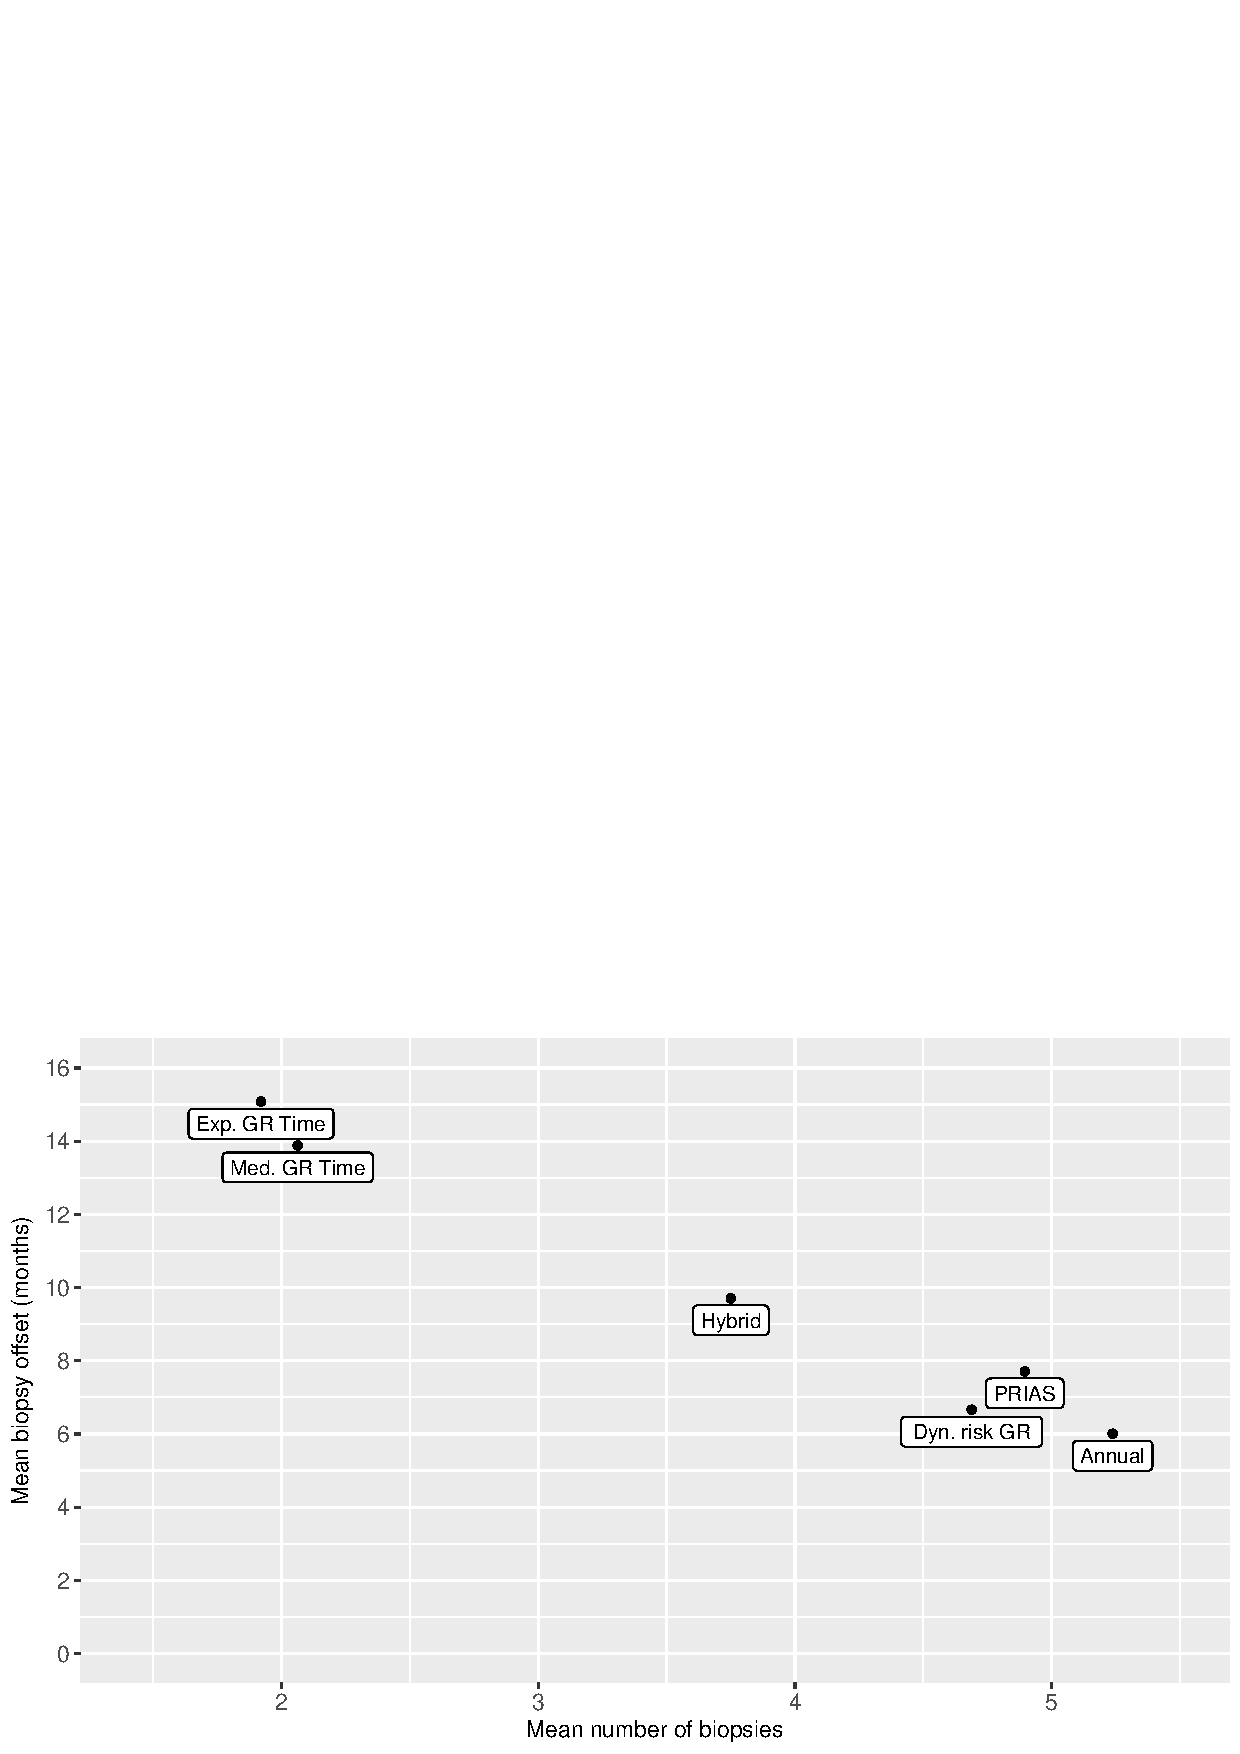
\includegraphics[width=\columnwidth]{images/sim_study/meanNbVsOffset_all.png}}
	\caption{Estimated mean number of biopsies and mean offset (months) for the 7 scheduling methods using all patients. Method names are abbreviated for ease of graphing.}
	\label{fig : meanNbVsOffset}
\end{figure}

\begin{table}
\caption{Pooled estimates of mean and variance of number of biopsies and offset for all patients.}
\label{table : sim_study_pooled_estimates}
\begin{tabular}{lrrrr}
\Hline
Schedule          & $E[N^{bS}]$ & $E[O^{S}]$ & $\mbox{var}[N^{bS}]$ & $\mbox{var}[O^S]$ \\  \hline
Annual & 5.23           & 6.00               & 6.42          & 11.87             \\
PRIAS & 4.85           & 8.46               & 5.52          & 74.22             \\
Expected time of GR & 1.92           & 15.06              & 1.42          & 146.31          \\
Median time of GR  & 2.06           & 13.89              & 2.00          & 139.73            \\
$\text{F}_1$-Score  & 4.68           & 6.65               & 4.80          & 18.83             \\
Mixed approach & 3.76          & 9.74               & 2.88          & 58.35             \\
\hline
\end{tabular}
\end{table}

We observe that the PRIAS schedule performs more or less the same as annual schedule. Despite this the latter may be preferred over PRIAS since it conducts only 0.38 biopsies more on average, however unlike PRIAS it has very low variance of offset, thus guaranteeing early detection for everyone. If we compare the PRIAS schedule with dynamic risk of GR based schedules, we can see that the schedule where $\kappa$ is chosen after maximizing $\text{F}_1$-Score, performs better than in PRIAS schedule in all aspects. The schedule where $\kappa$ is chosen after maximizing Youden's $J$ has a very large $\mbox{var}[O^S]$ and hence is not preferable over PRIAS. The mixed approach combines the benefits of methods with low $E[N^{bS}]$ and $\mbox{var}[N^{bS}]$, and those methods with low $E[O^{S}]$ and $\mbox{var}[O^S]$. It conducts 1.5 less biopsies than annual schedule on average and at 9.7 months the mean offset is less than an year.

\begin{table}
\caption{Pooled estimates of mean and variance of number of biopsies and offset for subgroup $G_1$.}
\label{table : sim_study_pooled_estimates_G1}
\begin{tabular}{lrrrrr}
\Hline
Schedule           & Total Patients & $E[N^{bS}]$ & $E[O^{S}]$ & $\mbox{var}[N^{bS}]$ & $\mbox{var}[O^S]$ \\  \hline
Annual              & 21004                  & 4.306           & 6.024               & 9.788          & 11.747             \\
PRIAS              & 21004                  & 4.032           & 7.951               & 8.221          & 63.528             \\
Expected time of GR & 21001                  & 1.922           & 15.114              & 1.441          & 149.167            \\
Median time of GR  & 20937                  & 2.068           & 13.87               & 1.999          & 138.396            \\
$\text{F}_1$-Score           & 21061                  & 4.689           & 6.648               & 4.863          & 18.745             \\
Mixed approach     & 21004                  & 3.252           & 10.361              & 4.611          & 73.781             \\
\hline
\end{tabular}
\end{table}

\begin{table}
\caption{Pooled estimates of mean and variance of number of biopsies and offset for subgroup $G_2$.}
\label{table : sim_study_pooled_estimates_G2}
\begin{tabular}{lrrrrr}
\Hline
Schedule           & Total Patients & $E[N^{bS}]$ & $E[O^{S}]$ & $\mbox{var}[N^{bS}]$ & $\mbox{var}[O^S]$ \\  \hline
Annual              & 21160                  & 5.181           & 5.95                & 4.567          & 12.03              \\
PRIAS              & 21160                  & 4.817           & 8.569               & 3.98           & 75.716             \\
Expected time of GR & 21151                  & 1.927           & 15.078              & 1.447          & 144.333            \\
Median time of GR  & 21189                  & 2.062           & 13.947              & 1.994          & 140.633            \\
$\text{F}_1$-Score           & 21133                  & 4.666           & 6.663               & 4.726          & 18.956             \\
Mixed approach     & 21160                  & 3.702           & 10.359              & 1.869          & 60.415             \\
\hline
\end{tabular}
\end{table}

\begin{table}
\caption{Pooled estimates of mean and variance of number of biopsies and offset for subgroup $G_3$.}
\label{table : sim_study_pooled_estimates_G3}
\begin{tabular}{lrrrrr}
\Hline
Schedule           & Total Patients & $E[N^{bS}]$ & $E[O^{S}]$ & $\mbox{var}[N^{bS}]$ & $\mbox{var}[O^S]$ \\  \hline
Annual              & 21222                  & 6.214           & 6.03                & 3.118          & 11.851             \\
PRIAS              & 21222                  & 5.717           & 8.866               & 2.977          & 82.915             \\
Expected time of GR  & 21234                  & 1.921           & 15.006              & 1.375          & 145.426            \\
Median time of GR   & 21260                  & 2.07            & 13.879              & 2.016          & 140.14             \\
Youden's $J$              & 21202                  & 4.541           & 8.02                & 4.061          & 112.559             \\
Mixed approach     & 21222                  & 4.33            & 8.521               & 1.581          & 38.586             \\
\hline
\end{tabular}
\end{table}

We next check the performance of these methods for each of the 3 subgroups $G_1, G_2$ and $G_3$. Estimates of $E[N^{bS}]$, $\mbox{var}[N^{bS}]$, $E[O^S]$ and $\mbox{var}[O^S]$ for the 3 subgroups are presented in Table \ref{table : sim_study_pooled_estimates_G1}, Table \ref{table : sim_study_pooled_estimates_G2} and Table \ref{table : sim_study_pooled_estimates_G3}. We observe that all of the schedules which are based on personalized methods, i.e. expected time of GR, median time of GR and dynamic risk of GR based schedules perform the same across the subgroups, with trivial differences in estimates. On the other hand, the annual schedule conducts 6 biopsies on average for patients in $G_3$ as compared to 4 for patients in $G_1$. It also has $\mbox{var}[N^{bS}]$ 3 times more for patients in $G_1$ compared to $G_3$. This can be attributed to the former having higher variance in GR times. However for annual schedule the $E[O^S]$ and $\mbox{var}[O^S]$ remain almost the same in all groups and it always detects GR within an year of the occurrence. The PRIAS schedule differs for the 3 subgroups as well. For number of biopsies the dynamics are similar to that of annual schedule. However for offset, the PRIAS schedule has high $E[O^S]$ and $\mbox{var}[O^S]$ for patients from $G_3$, i.e. patients who obtain GR later. As for the mixed approach, we observe that it conducts more biopsies on average for patients from $G_3$, however it also has the least $E[O^S]$, $\mbox{var}[O^S]$ and $\mbox{var}[N^{bS}]$ for the same group.

To assess the methods further, we combined data from all of the 63386 patients, and also plotted the box plots for number of biopsies and offset in Figure \ref{fig : nbBoxPlot} and Figure \ref{fig : offsetBoxPlot} respectively. Based on the combined data, we observe that both expected and median failure time of GR based schedules have 91.7\% and 92.5\% of patients below offset cutoff of 36 months, respectively. They also have 80.5\% and 82.3\% of patients below a cutoff of 24 months. Thus they seem to be quite practical. The mixed approach offers another practically viable solution, since neither it has large $\mbox{var}[N^{bS}]$, nor $\mbox{var}[O^S]$. The estimated $E[N^{bS}]$ is 3.8 and the estimated $E[O^S]$ is 9.7 months. For 99.9\% patients it has an offset below 36 months and for 95\% patients it has an offset below 24 months. Given this offset and the fact that it conducts much less biopsies than PRIAS schedule, annual schedule, and dynamic risk of GR based schedules, it is preferable over them.

\textbf{}

\clearpage
\printbibliography

\appendix

% !TEX root =  ../main.tex 

\section{Appendix}

\subsection{Personalized schedules for repeat biopsies}
In this section we present the derivations for Equation \ref{eq : expected_time_survprob} and Equation \ref{eq : var_time_survprob}. To this end, we first expand the formula for dynamic survival probability presented in Equation \ref{eq : dynamic_surv_prob}.
\begin{equation}
\label{eq : dyn_surv_prob_expanded}
\begin{split}
\pi_j(u \mid t, s) &= \mbox{Pr}\big\{T^*_j \geq u \mid  T^*_j >t, \mathcal{Y}_j(s\big\}, D_n)\\
&= \int \int \mbox{Pr}\big\{T^*_j \geq u \mid  T^*_j >t, \boldsymbol{b}_j,\boldsymbol{\theta}\big\} p\big(\boldsymbol{b}_j \mid T^*_j>t, \mathcal{Y}_j(s), \boldsymbol{\theta}\big)p\big(\boldsymbol{\theta} \mid \mathcal{D}_n\big) \diff \boldsymbol{b}_j \diff \boldsymbol{\theta}\\
&= \int \int \frac{\exp\big\{-H_j(u | \boldsymbol{b}_j, \boldsymbol{\theta})\big\}}{\exp\big\{-H_j(t | \boldsymbol{b}_j, \boldsymbol{\theta})\big\}} p\big(\boldsymbol{b}_j \mid T^*_j>t, \mathcal{Y}_j(s), \boldsymbol{\theta}\big)p\big(\boldsymbol{\theta} \mid \mathcal{D}_n\big) \diff \boldsymbol{b}_j \diff \boldsymbol{\theta}
\end{split}
\end{equation}
where $H_j(u | \boldsymbol{b}_j, \boldsymbol{\theta}) = \int_0^u h_i(s \mid \boldsymbol{b}_j, \boldsymbol{\theta}\big)\diff s$ is the cumulative hazard up to time point $u$.

\subsubsection{Derivation of Equation \ref{eq : expected_time_survprob}}
\label{subsubsec : deriv_eq_7}
\begin{equation*}
\begin{split}
E_g[T^*_j] &= \int_t^{\infty} T^*_j g(T^*_j)\diff T^*_j\\
\text{Using integration by parts, wherein} & \frac{\diff \big\{-\pi_j(T^*_j \mid t, s)\big\}}{\diff T^*_j} = g(T^*_j)\\
&= \Big[-T^*_j\pi_j(T^*_j \mid t, s)\Big]_t^\infty + \int_t^{\infty} \pi_j(T^*_j \mid t, s) \frac{\diff (T^*_j)}{\diff T^*_j} \diff T^*_j\\
&= t \pi_j(t \mid t, s) - \lim_{T^*_j\to \infty}T^*_j \pi_j(T^*_j \mid t, s) + \int_t^{\infty} \pi_j(T^*_j \mid t, s) \diff T^*_j\\
\end{split}
\end{equation*}
where $\pi_j(t \mid t, s) = \mbox{Pr}\big\{T^*_j \geq t \mid  T^*_j >t, \mathcal{Y}_j(s), D_n\big\} = 1$. As for $\lim_{T^*_j\to \infty}T^*_j \pi_j(T^*_j \mid t, s)$, the limit can be interchanged with the integral in Equation \ref{eq : dyn_surv_prob_expanded}, because as $T^*_j\to \infty$ the integrand in the equation converges uniformly on the domain of $(\boldsymbol{b}_j, \boldsymbol{\theta}\big)$. Thus,
\begin{equation*}
\begin{split}
\lim_{T^*_j\to \infty}T^*_j \pi_j(T^*_j \mid t, s) &=  \int \int \lim_{T^*_j\to \infty} \frac{T^*_j}{\exp\big\{H_j(T^*_j | \boldsymbol{b}_j, \boldsymbol{\theta})\big\}} \frac{p\big(\boldsymbol{b}_j \mid T^*_j>t, \mathcal{Y}_j(s), \boldsymbol{\theta}\big)p\big(\boldsymbol{\theta} \mid \mathcal{D}_n\big)}{\exp\big\{-H_j(t | \boldsymbol{b}_j, \boldsymbol{\theta})\big\}}  \diff \boldsymbol{b}_j \diff \boldsymbol{\theta}\\
\text{Using L'Hospital's rule}\\
\lim_{T^*_j\to \infty}T^*_j \pi_j(T^*_j \mid t, s) &=  \int \int \frac{1}{\lim_{T^*_j\to \infty} \exp\{H_j(T^*_j | \boldsymbol{b}_j, \boldsymbol{\theta}\big)\}H'_j(T^*_j | \boldsymbol{b}_j, \boldsymbol{\theta}\big)} \frac{p\big(\boldsymbol{b}_j \mid T^*_j>t, \mathcal{Y}_j(s), \boldsymbol{\theta}\big)p\big(\boldsymbol{\theta} \mid \mathcal{D}_n\big)}{\exp\{-H_j(t | \boldsymbol{b}_j, \boldsymbol{\theta}\big)\}} \diff \boldsymbol{b}_j \diff \boldsymbol{\theta}\\
&= \int \int 0 \frac{p\big(\boldsymbol{b}_j \mid T^*_j>t, \mathcal{Y}_j(s), \boldsymbol{\theta}\big)p\big(\boldsymbol{\theta} \mid \mathcal{D}_n\big)}{\exp\big\{-H_j(t | \boldsymbol{b}_j, \boldsymbol{\theta})\big\}}  \diff \boldsymbol{b}_j \diff \boldsymbol{\theta}\\
&= 0
\end{split}
\end{equation*}

In light of these results, we obtain:
\begin{equation*}
E_g[T^*_j] = t + \int_t^{\infty} \pi_j(T^*_j \mid t, s) \diff T^*_j\\
\end{equation*}

\subsubsection{Derivation of Equation \ref{eq : var_time_survprob}}
Since $\mbox{var}_g[T^*_j] = E_g[\{T^*_j\}^2] - E_g[T^*_j]^2$, we first show the derivation for $E_g[(T^*_j)^2]$.
\begin{equation*}
\begin{split}
E_g[(T^*_j)^2] &= \int_t^{\infty} (T^*_j)^2 g(T^*_j)\diff T^*_j\\
\text{Using integration by parts, wherein} & \frac{\diff \big\{-\pi_j(T^*_j \mid t, s)\big\}}{\diff T^*_j} = g(T^*_j)\\
E_g\big[\{T^*_j\}^2\big] &= \Big[-\{T^*_j\}^2\pi_j(T^*_j \mid t, s)\Big]_t^\infty + \int_t^{\infty} \pi_j(T^*_j \mid t, s) \frac{\diff (T^*_j)^2}{\diff T^*_j} \diff T^*_j\\
&= t^2 \pi_j(t \mid t, s) - \lim_{T^*_j\to \infty}(T^*_j)^2 \pi_j(T^*_j \mid t, s) + 2 \int_t^{\infty} T^*_j \pi_j(T^*_j \mid t, s) \diff T^*_j\\
&= t^2 + 2 \int_t^{\infty} T^*_j \pi_j(T^*_j \mid t, s) \diff T^*_j
\end{split}
\end{equation*}
Therefore,
\begin{equation*}
\begin{split}
\mbox{var}_g[T^*_j] &= t^2 + 2 \int_t^{\infty} T^*_j \pi_j(T^*_j \mid t, s) \diff T^*_j - \bigg[t^2 +  \Big\{\int_t^\infty \pi_j(T^*_j \mid t, s) \diff T^*_j \Big\}^2 + 2t\int_t^\infty \pi_j(T^*_j \mid t, s) \diff T^*_j \bigg]\\
&=2 \int_t^{\infty} (T^*_j - t) \pi_j(T^*_j \mid t, s) \diff T^*_j -  \Big\{\int_t^\infty \pi_j(T^*_j \mid t, s) \diff T^*_j \Big\}^2
\end{split}
\end{equation*}

\subsection{Simulation study}
This section presents the figures and tables for related to the simulation study results from Section \ref{sec: simulation_study}. More specifically:

\begin{itemize}
  \item Figure \ref{fig : meanNbVsOffset_G1}, Figure \ref{fig : meanNbVsOffset_G2} and Figure \ref{fig : meanNbVsOffset_G3} show plots of average number of biopsies against average offset for each of the 7 scheduling methods present in the simulation study.
  \item Figure \ref{fig : nbBoxPlot_G1} and Figure \ref{fig : offsetBoxPlot_G1} show boxplots of number of biopsies and offset for each of the 6 scheduling methods for the patients in subgroup $G_1$. Similar plots for subgroup $G_2$ and $G_3$ are shown in Figure \ref{fig : nbAndOffsetBoxPlot_G2} and Figure \ref{fig : nbAndOffsetBoxPlot_G3} respectively.
  \item Figure \ref{fig : nbMeanBoxPlot_all} and Figure \ref{fig : offsetMeanBoxPlot_all} show the variation in estimated mean number of biopsies and estimated mean offset computed during the 254 simulations, for patients from all subgroups. The same plots for each of the subgroups are shown in Figure \ref{fig : nbAndOffsetMeanBoxPlot_G1}, Figure \ref{fig : nbAndOffsetMeanBoxPlot_G2} and Figure \ref{fig : nbAndOffsetMeanBoxPlot_G3}.
\end{itemize} 

\begin{figure}[!htb]
    \centering
    \captionsetup{justification=centering}
     \begin{subfigure}[b]{0.45\textwidth}
        \includegraphics[width=\textwidth]{images/sim_study/meanNbVsOffset_scale_4.png}
		\caption{Plot for subgroup $G_1$}
		\label{fig : meanNbVsOffset_G1}
    \end{subfigure}
    \begin{subfigure}[b]{0.45\textwidth}
		\includegraphics[width=\textwidth]{images/sim_study/meanNbVsOffset_scale_5.png}
		\caption{Plot for subgroup $G_2$}
		\label{fig : meanNbVsOffset_G2}
    \end{subfigure}  
    \begin{subfigure}[b]{0.45\textwidth}
		\includegraphics[width=\textwidth]{images/sim_study/meanNbVsOffset_scale_6.png}
		\caption{Plot for subgroup $G_3$}
		\label{fig : meanNbVsOffset_G3}
    \end{subfigure}      
    \caption{Estimated mean number of biopsies and mean offset (months) for the 7 scheduling methods for the 3 sub-groups. Method names are abbreviated for ease of graphing.}
\end{figure}

\begin{figure}[!htb]
    \centering
    \captionsetup{justification=centering}
     \begin{subfigure}[b]{0.45\textwidth}
        \includegraphics[width=\textwidth]{images/sim_study/nbBoxPlot_scale_4.png}
        \caption{Boxplot for number of biopsies.}
        \label{fig : nbBoxPlot_G1}
    \end{subfigure}
    \begin{subfigure}[b]{0.45\textwidth}
        \includegraphics[width=\textwidth]{images/sim_study/offsetBoxPlot_scale_4.png}
        \caption{Boxplot for offset (months)}
        \label{fig : offsetBoxPlot_G1}
    \end{subfigure}      
    \caption{Boxplot for number of biopsies and offset (months), for all patients in subgroup $G_1$ across all simulations. Method names are abbreviated for ease of graphing.}
    \label{fig : nbAndOffsetBoxPlot_G1}
\end{figure}

\begin{figure}[!htb]
    \centering
    \captionsetup{justification=centering}
     \begin{subfigure}[b]{0.45\textwidth}
        \includegraphics[width=\textwidth]{images/sim_study/nbBoxPlot_scale_5.png}
        \caption{Boxplot for number of biopsies.}
        \label{fig : nbBoxPlot_G2}
    \end{subfigure}
    \begin{subfigure}[b]{0.45\textwidth}
        \includegraphics[width=\textwidth]{images/sim_study/offsetBoxPlot_scale_5.png}
        \caption{Boxplot for offset (months)}
        \label{fig : offsetBoxPlot_G2}
    \end{subfigure}      
    \caption{Boxplot for number of biopsies and offset (months), for all patients in subgroup $G_2$ across all simulations. Method names are abbreviated for ease of graphing.}
     \label{fig : nbAndOffsetBoxPlot_G2}
\end{figure}

\begin{figure}[!htb]
    \centering
    \captionsetup{justification=centering}
     \begin{subfigure}[b]{0.45\textwidth}
        \includegraphics[width=\textwidth]{images/sim_study/nbBoxPlot_scale_6.png}
        \caption{Boxplot for number of biopsies.}
        \label{fig : nbBoxPlot_G3}
    \end{subfigure}
    \begin{subfigure}[b]{0.45\textwidth}
        \includegraphics[width=\textwidth]{images/sim_study/offsetBoxPlot_scale_6.png}
        \caption{Boxplot for offset (months)}
        \label{fig : offsetBoxPlot_G3}
    \end{subfigure}      
    \caption{Boxplot for number of biopsies and offset (months), for all patients in subgroup $G_3$ across all simulations. Method names are abbreviated for ease of graphing.}
     \label{fig : nbAndOffsetBoxPlot_G3}
\end{figure}

\begin{figure}[!htb]
    \centering
    \captionsetup{justification=centering}
     \begin{subfigure}[b]{0.45\textwidth}
        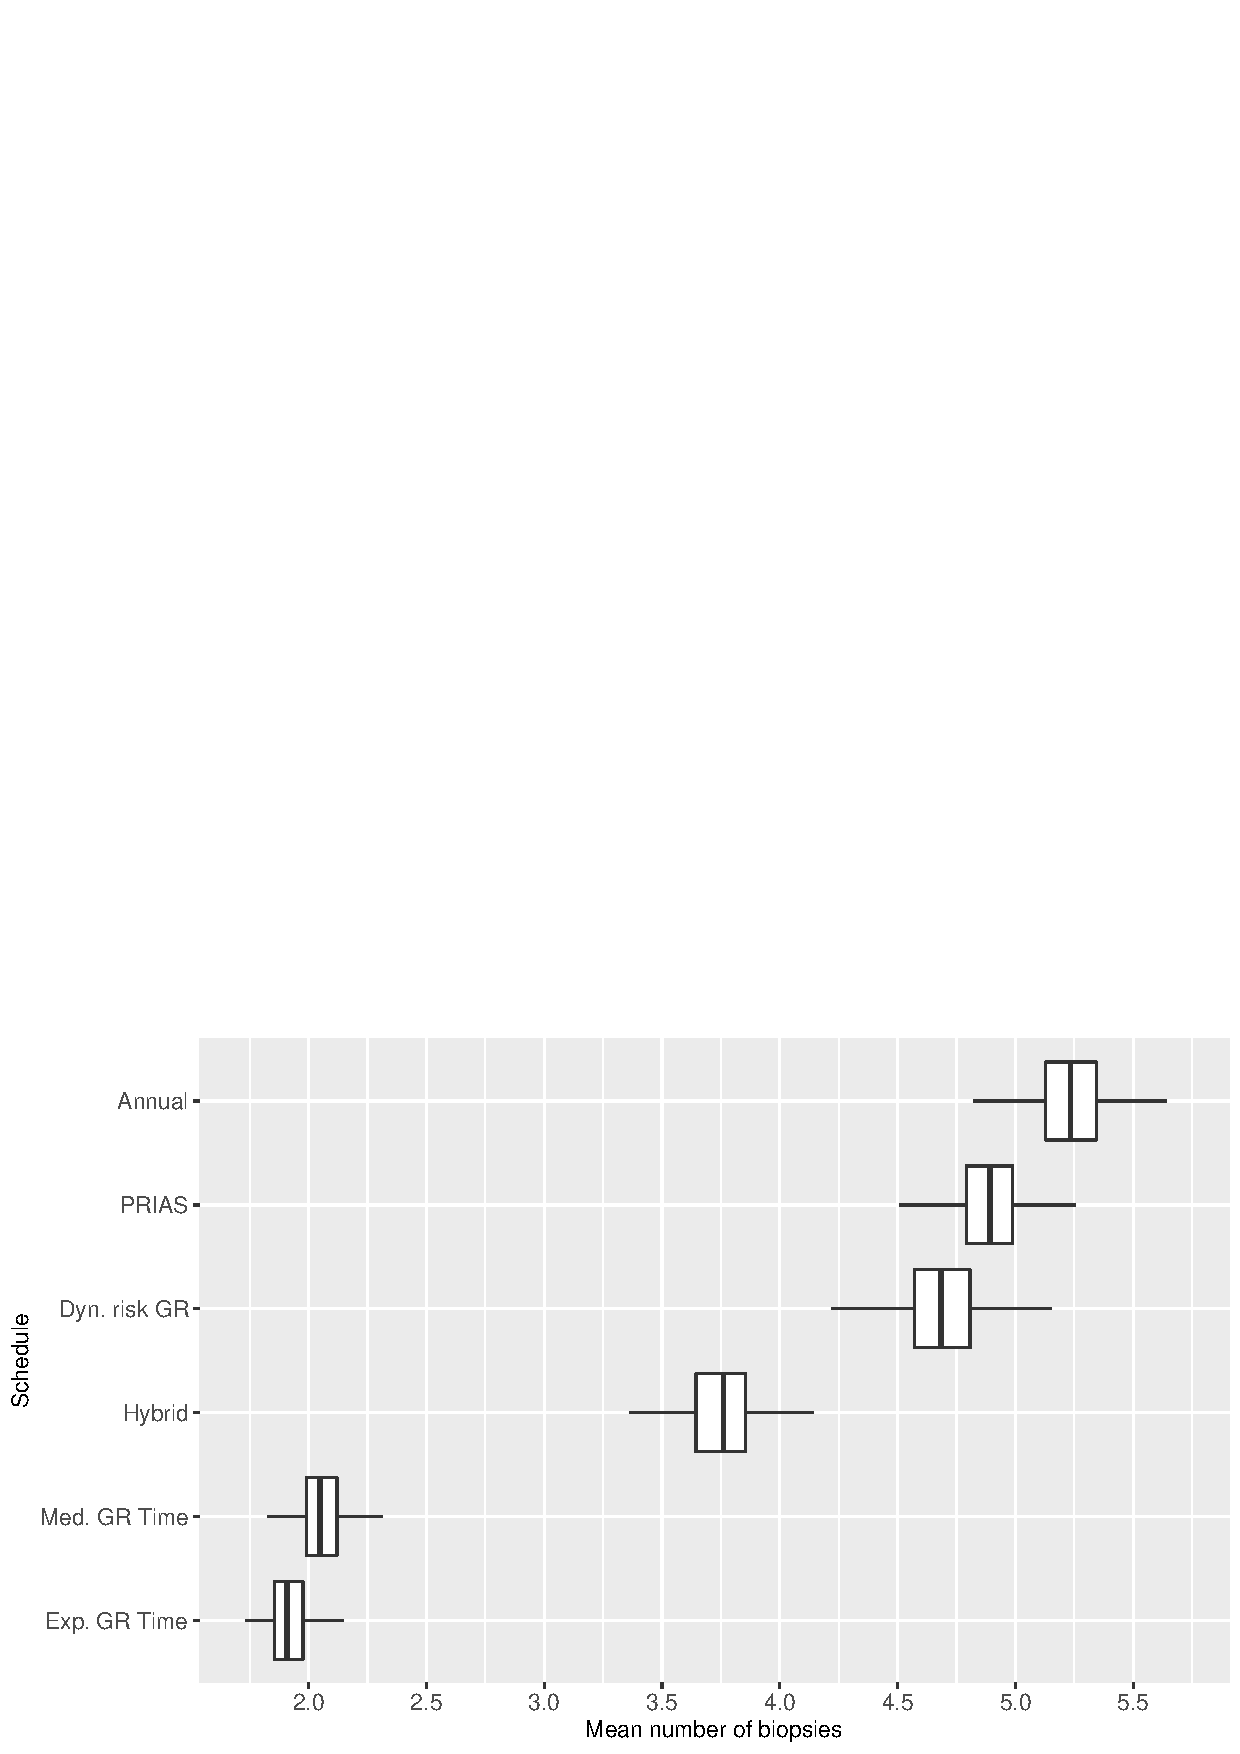
\includegraphics[width=\textwidth]{images/sim_study/nbMeanBoxPlot_all.png}
        \caption{Boxplot for mean number of biopsies.}
        \label{fig : nbMeanBoxPlot_all}
    \end{subfigure}
    \begin{subfigure}[b]{0.45\textwidth}
        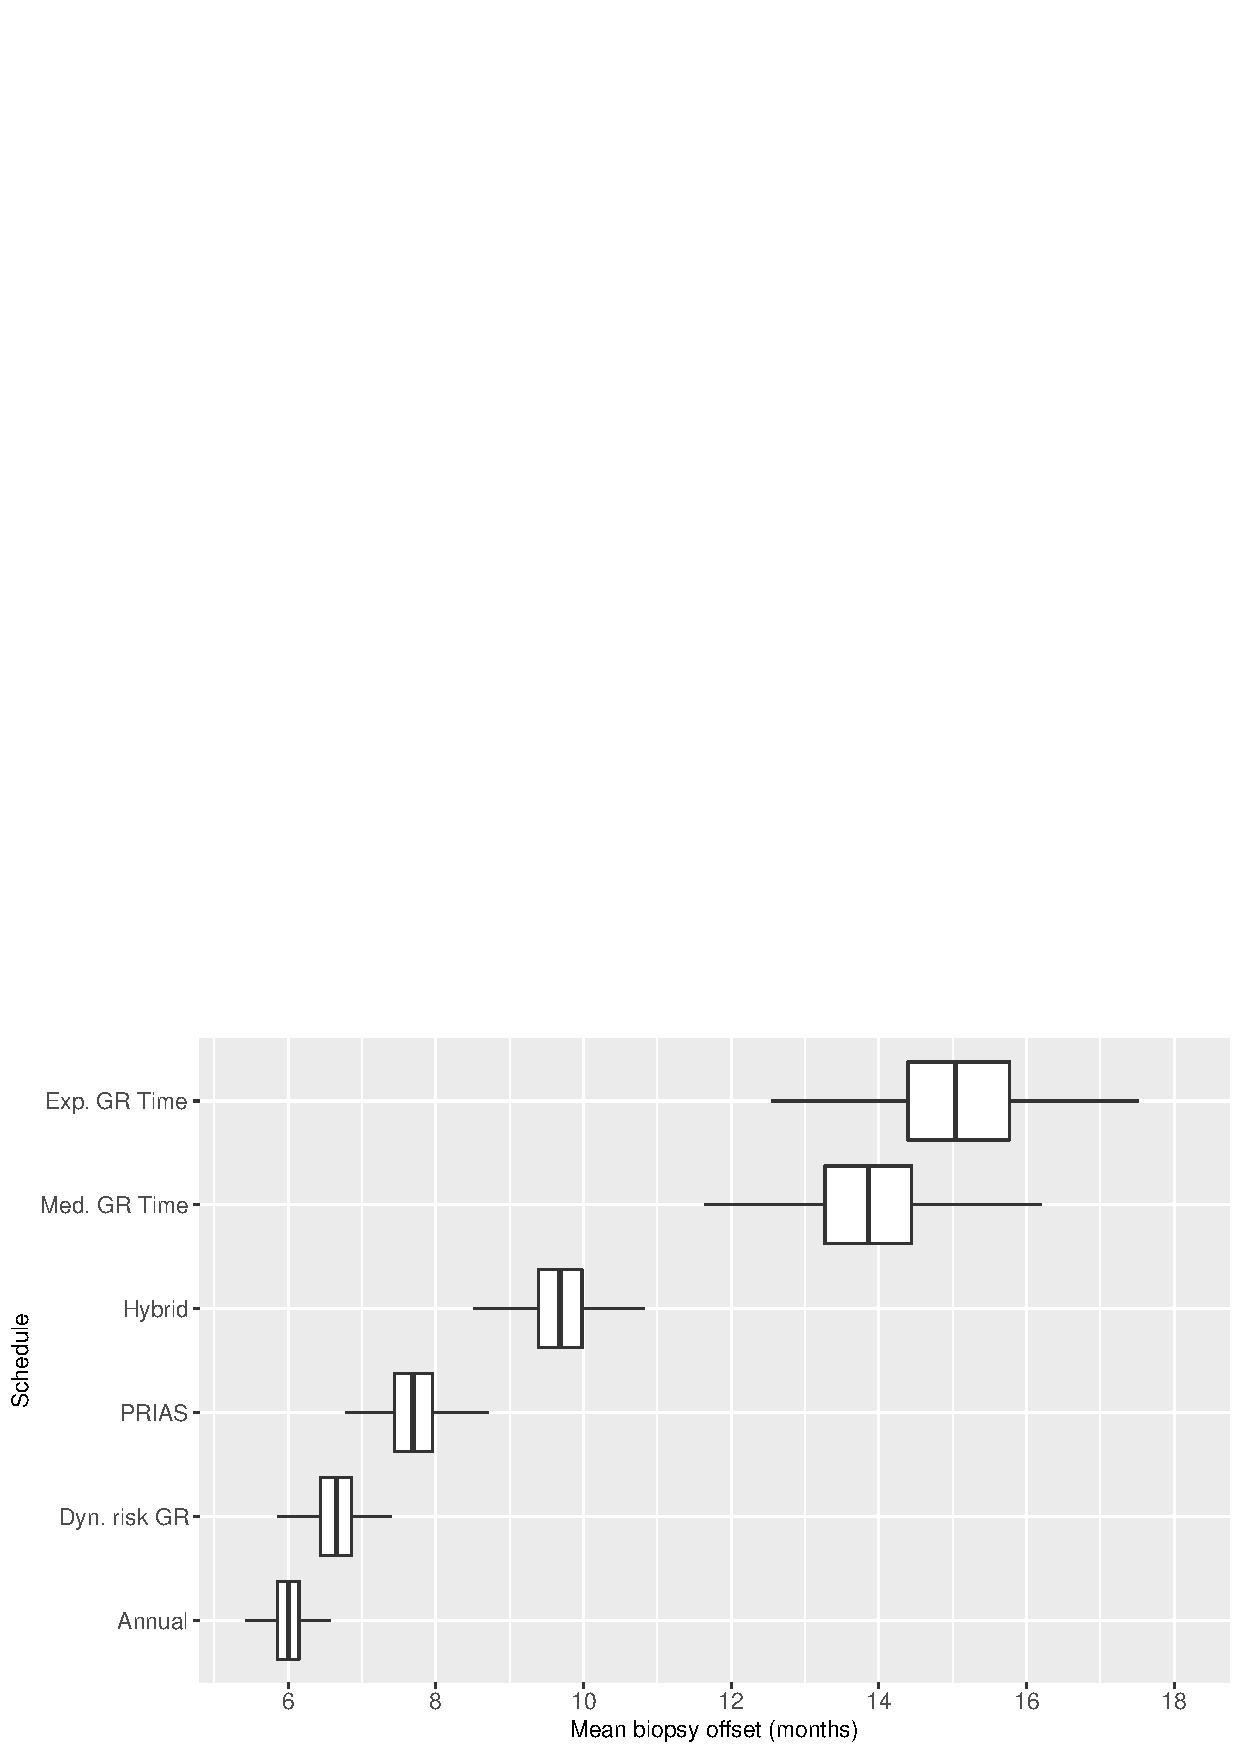
\includegraphics[width=\textwidth]{images/sim_study/offsetMeanBoxPlot_all.png}
        \caption{Boxplot for mean offset (months)}
        \label{fig : offsetMeanBoxPlot_all}
    \end{subfigure}      
    \caption{Boxplot showing variation in mean number of biopsies and mean offset (months) for all of the patients across the 254 simulations.}
\end{figure}

\begin{figure}[!htb]
    \centering
    \captionsetup{justification=centering}
     \begin{subfigure}[b]{0.45\textwidth}
        \includegraphics[width=\textwidth]{images/sim_study/nbMeanBoxPlot_scale_4.png}
        \caption{Boxplot for mean number of biopsies.}
        \label{fig : nbMeanBoxPlot_G1}
    \end{subfigure}
    \begin{subfigure}[b]{0.45\textwidth}
        \includegraphics[width=\textwidth]{images/sim_study/offsetMeanBoxPlot_scale_4.png}
        \caption{Boxplot for mean offset (months)}
        \label{fig : offsetMeanBoxPlot_G1}
    \end{subfigure}      
    \caption{Boxplot showing variation in mean number of biopsies and mean offset (months) for patients in subgroup $G_1$ across the 254 simulations.}
    \label{fig : nbAndOffsetMeanBoxPlot_G1}
\end{figure}

\begin{figure}[!htb]
    \centering
    \captionsetup{justification=centering}
     \begin{subfigure}[b]{0.45\textwidth}
        \includegraphics[width=\textwidth]{images/sim_study/nbMeanBoxPlot_scale_5.png}
        \caption{Boxplot for mean number of biopsies.}
        \label{fig : nbMeanBoxPlot_G2}
    \end{subfigure}
    \begin{subfigure}[b]{0.45\textwidth}
        \includegraphics[width=\textwidth]{images/sim_study/offsetMeanBoxPlot_scale_5.png}
        \caption{Boxplot for mean offset (months)}
        \label{fig : offsetMeanBoxPlot_G2}
    \end{subfigure}      
    \caption{Boxplot showing variation in mean number of biopsies and mean offset (months) for patients in subgroup $G_2$ across the 254 simulations.}
    \label{fig : nbAndOffsetMeanBoxPlot_G2}
\end{figure}

\begin{figure}[!htb]
    \centering
    \captionsetup{justification=centering}
     \begin{subfigure}[b]{0.45\textwidth}
        \includegraphics[width=\textwidth]{images/sim_study/nbMeanBoxPlot_scale_6.png}
        \caption{Boxplot for mean number of biopsies.}
        \label{fig : nbMeanBoxPlot_G3}
    \end{subfigure}
    \begin{subfigure}[b]{0.45\textwidth}
        \includegraphics[width=\textwidth]{images/sim_study/offsetMeanBoxPlot_scale_6.png}
        \caption{Boxplot for mean offset (months)}
        \label{fig : offsetMeanBoxPlot_G3}
    \end{subfigure}      
    \caption{Boxplot showing variation in mean number of biopsies and mean offset (months) for patients in subgroup $G_3$ across the 254 simulations.}
    \label{fig : nbAndOffsetMeanBoxPlot_G3}
\end{figure}

\end{document}